\pdfoutput=1
\documentclass[11pt]{article}
\usepackage[T1]{fontenc}
\usepackage[utf8]{inputenc}
\usepackage{mathpazo}
\usepackage[scaled=0.92]{helvet}
\usepackage{amsmath,amssymb}
\usepackage[a4paper,margin=2.5cm,headheight=14pt]{geometry}
\usepackage{graphicx}
\usepackage{booktabs,tabularx,threeparttable,longtable,float}
\usepackage[font=small,labelfont=bf,labelsep=colon]{caption}
\usepackage{microtype}
\usepackage{enumitem}
\usepackage{xcolor}
\usepackage[most]{tcolorbox}
\usepackage{fancyhdr}
\usepackage[square,sort,comma,authoryear]{natbib}
\usepackage[colorlinks=true,linkcolor={blue!45!black},citecolor={blue!45!black},urlcolor={blue!45!black}]{hyperref}
\usepackage{url}
\def\UrlBreaks{\do\/\do-\do_\do.}

% Generated by model/make_numbers.py from results.json -- do not edit.
\newcommand{\AbuBattery}{999}
\newcommand{\AbuChargerGW}{4\,425}
\newcommand{\AbuCum}{4.66~billion}
\newcommand{\AbuHHshare}{37}
\newcommand{\AbuKwhFifty}{2\,455}
\newcommand{\AbuKwhForty}{2\,375}
\newcommand{\AbuKwhThirty}{2\,015}
\newcommand{\AbuKwhThirtyFive}{2\,204}
\newcommand{\AbuOffFifty}{349}
\newcommand{\AbuOffForty}{256}
\newcommand{\AbuOffThirty}{1.96}
\newcommand{\AbuOffThirtyFive}{109}
\newcommand{\AbuPeakCN}{405}
\newcommand{\AbuPeakCNThirtyFive}{130.4}
\newcommand{\AbuPeakCNconc}{708}
\newcommand{\AbuPeakSum}{1\,012}
\newcommand{\AbuPeakSumMan}{725}
\newcommand{\AbuPeakWorld}{728}
\newcommand{\AbuQmax}{250~million}
\newcommand{\AbuQmaxM}{250}
\newcommand{\AbuShipFifty}{250~million}
\newcommand{\AbuShipForty}{250~million}
\newcommand{\AbuShipThirty}{17~million}
\newcommand{\AbuShipThirtyFive}{247~million}
\newcommand{\AbuStockFifty}{2.21~billion}
\newcommand{\AbuStockForty}{1.70~billion}
\newcommand{\AbuStockThirty}{20~million}
\newcommand{\AbuStockThirtyFive}{794~million}
\newcommand{\AbuStockThirtyFiveTxt}{794~million}
\newcommand{\AbuTWhFifty}{5\,427}
\newcommand{\AbuTWhForty}{3\,859}
\newcommand{\AbuTWhThirty}{25.0}
\newcommand{\AbuTWhThirtyFive}{1\,519}
\newcommand{\AbuVehRatio}{2.59}
\newcommand{\AbuVehYear}{2032}
\newcommand{\AbuWorldShare}{16.2}
\newcommand{\AbuWorldShareThirtyFive}{4.52}
\newcommand{\Abuk}{1.43}
\newcommand{\Abukpct}{317}
\newcommand{\Abutm}{2032}
\newcommand{\AccBattery}{639}
\newcommand{\AccBofASForty}{0.95}
\newcommand{\AccBofAThirty}{0.58}
\newcommand{\AccBofAThirtyFive}{1.36}
\newcommand{\AccChargerGW}{2\,141}
\newcommand{\AccCum}{1.86~billion}
\newcommand{\AccHHshare}{35}
\newcommand{\AccKwhFifty}{2\,006}
\newcommand{\AccKwhForty}{1\,970}
\newcommand{\AccKwhThirty}{1\,888}
\newcommand{\AccKwhThirtyFive}{1\,939}
\newcommand{\AccOffFifty}{166}
\newcommand{\AccOffForty}{38.1}
\newcommand{\AccOffThirty}{0.15}
\newcommand{\AccOffThirtyFive}{3.21}
\newcommand{\AccPeakCN}{160}
\newcommand{\AccPeakCNThirtyFive}{3.8}
\newcommand{\AccPeakCNconc}{280}
\newcommand{\AccPeakSum}{400}
\newcommand{\AccPeakSumMan}{287}
\newcommand{\AccPeakWorld}{288}
\newcommand{\AccQmax}{160~million}
\newcommand{\AccQmaxM}{160}
\newcommand{\AccShipFifty}{160~million}
\newcommand{\AccShipForty}{106~million}
\newcommand{\AccShipThirty}{692\,000}
\newcommand{\AccShipThirtyFive}{14~million}
\newcommand{\AccStockFifty}{1.07~billion}
\newcommand{\AccStockForty}{285~million}
\newcommand{\AccStockThirty}{1.3~million}
\newcommand{\AccStockThirtyFive}{26~million}
\newcommand{\AccTWhFifty}{2\,117}
\newcommand{\AccTWhForty}{475}
\newcommand{\AccTWhThirty}{1.83}
\newcommand{\AccTWhThirtyFive}{39.5}
\newcommand{\AccVehRatio}{1.66}
\newcommand{\AccVehYear}{2040}
\newcommand{\AccWorldShare}{6.3}
\newcommand{\AccWorldShareThirtyFive}{0.12}
\newcommand{\Acck}{0.61}
\newcommand{\Acckpct}{84}
\newcommand{\Acctm}{2039}
\newcommand{\AnaRatio}{931}
\newcommand{\AnaStockFifty}{808\,000}
\newcommand{\AnaTWhFifty}{1.4}
\newcommand{\AnaTWhThirtyFive}{0.38}
\newcommand{\ConBattery}{31}
\newcommand{\ConChargerGW}{111}
\newcommand{\ConCum}{122~million}
\newcommand{\ConHHshare}{6}
\newcommand{\ConKwhFifty}{1\,873}
\newcommand{\ConKwhForty}{1\,845}
\newcommand{\ConKwhThirty}{1\,809}
\newcommand{\ConKwhThirtyFive}{1\,827}
\newcommand{\ConOffFifty}{8.69}
\newcommand{\ConOffForty}{4.95}
\newcommand{\ConOffThirty}{0.12}
\newcommand{\ConOffThirtyFive}{1.36}
\newcommand{\ConPeakCN}{7.7}
\newcommand{\ConPeakCNThirtyFive}{1.4}
\newcommand{\ConPeakCNconc}{13}
\newcommand{\ConPeakSum}{19}
\newcommand{\ConPeakSumMan}{14}
\newcommand{\ConPeakWorld}{14}
\newcommand{\ConQmax}{7.9~million}
\newcommand{\ConQmaxM}{8}
\newcommand{\ConShipFifty}{7.9~million}
\newcommand{\ConShipForty}{7.4~million}
\newcommand{\ConShipThirty}{500\,000}
\newcommand{\ConShipThirtyFive}{4.0~million}
\newcommand{\ConStockFifty}{55~million}
\newcommand{\ConStockForty}{34~million}
\newcommand{\ConStockThirty}{999\,000}
\newcommand{\ConStockThirtyFive}{10~million}
\newcommand{\ConTWhFifty}{103}
\newcommand{\ConTWhForty}{58.0}
\newcommand{\ConTWhThirty}{1.42}
\newcommand{\ConTWhThirtyFive}{15.8}
\newcommand{\ConVehRatio}{0.08}
\newcommand{\ConVehYear}{never}
\newcommand{\ConWorldShare}{0.3}
\newcommand{\ConWorldShareThirtyFive}{0.05}
\newcommand{\Conk}{0.54}
\newcommand{\Conkpct}{72}
\newcommand{\Contm}{2035}
\newcommand{\CoreSha}{7d26d8a81c94670e}
\newcommand{\Draws}{50\,000}
\newcommand{\EcoA}{0.174}
\newcommand{\EcoElecCostThreeSix}{303}
\newcommand{\EcoElecShareMax}{10.0}
\newcommand{\EcoElecShareMin}{0.4}
\newcommand{\EcoPminFifteenKSix}{0.14}
\newcommand{\EcoPminHundredKTwoFour}{0.71}
\newcommand{\EcoPminThirtyKThreeSix}{0.22}
\newcommand{\EcoPminTwoHundredKTwoFour}{1.31}
\newcommand{\LadA}{13.3}
\newcommand{\LadB}{14.1}
\newcommand{\LadBd}{$+$0.8}
\newcommand{\LadC}{20.5}
\newcommand{\LadCd}{$+$6.4}
\newcommand{\LadD}{21.0}
\newcommand{\LadDd}{$+$0.5}
\newcommand{\LadE}{20.2}
\newcommand{\LadEd}{$-$0.9}
\newcommand{\LadF}{22.9}
\newcommand{\LadFd}{$+$2.8}
\newcommand{\LegacyErr}{0.03}
\newcommand{\LegacyPeakPresent}{1.24}
\newcommand{\LegacyRY}{7.93~million}
\newcommand{\LegacyStock}{9.93~million}
\newcommand{\LegacyTWh}{13.3}
\newcommand{\LfA}{1\,255}
\newcommand{\LfB}{1\,144}
\newcommand{\LfBd}{$-$111}
\newcommand{\LfC}{991}
\newcommand{\LfCd}{$-$152}
\newcommand{\LfD}{1\,032}
\newcommand{\LfDd}{$+$41}
\newcommand{\LfE}{1\,348}
\newcommand{\LfEd}{$+$316}
\newcommand{\MCHCapped}{1.9}
\newcommand{\MCHFiftyFive}{377}
\newcommand{\MCHFiftyMed}{1\,727}
\newcommand{\MCHFiftyNinetyFive}{6\,356}
\newcommand{\MCHFiftySeventyFive}{3\,064}
\newcommand{\MCHFiftyTwentyFive}{921}
\newcommand{\MCHPctAbu}{92}
\newcommand{\MCHPctAcc}{59}
\newcommand{\MCHPctCon}{0}
\newcommand{\MCHPctRef}{39}
\newcommand{\MCHStockFive}{137~million}
\newcommand{\MCHStockMed}{594~million}
\newcommand{\MCHStockNinetyFive}{2.01~billion}
\newcommand{\MCHStockSeventyFive}{1.02~billion}
\newcommand{\MCHStockTwentyFive}{321~million}
\newcommand{\MCHThirtyFiveFive}{16.6}
\newcommand{\MCHThirtyFiveMed}{43.7}
\newcommand{\MCHThirtyFiveNinetyFive}{131}
\newcommand{\MCHThirtyFiveSeventyFive}{68.9}
\newcommand{\MCHThirtyFiveTwentyFive}{28.5}
\newcommand{\MCHTotalFive}{458}
\newcommand{\MCHTotalMed}{2\,084}
\newcommand{\MCHTotalNinetyFive}{7\,604}
\newcommand{\MCHTotalSeventyFive}{3\,677}
\newcommand{\MCHTotalTwentyFive}{1\,113}
\newcommand{\MCSCapped}{15.8}
\newcommand{\MCSFiftyFive}{70}
\newcommand{\MCSFiftyMed}{1\,276}
\newcommand{\MCSFiftyNinetyFive}{12\,656}
\newcommand{\MCSFiftySeventyFive}{3\,415}
\newcommand{\MCSFiftyTwentyFive}{419}
\newcommand{\MCSPctAbu}{85}
\newcommand{\MCSPctAcc}{63}
\newcommand{\MCSPctCon}{8}
\newcommand{\MCSPctRef}{52}
\newcommand{\MCSStockFive}{32~million}
\newcommand{\MCSStockMed}{552~million}
\newcommand{\MCSStockNinetyFive}{4.40~billion}
\newcommand{\MCSStockSeventyFive}{1.33~billion}
\newcommand{\MCSStockTwentyFive}{184~million}
\newcommand{\MCSThirtyFiveFive}{5.93}
\newcommand{\MCSThirtyFiveMed}{29.0}
\newcommand{\MCSThirtyFiveNinetyFive}{269}
\newcommand{\MCSThirtyFiveSeventyFive}{66.9}
\newcommand{\MCSThirtyFiveTwentyFive}{14.3}
\newcommand{\MCSTotalFive}{83}
\newcommand{\MCSTotalMed}{1\,546}
\newcommand{\MCSTotalNinetyFive}{15\,662}
\newcommand{\MCSTotalSeventyFive}{4\,137}
\newcommand{\MCSTotalTwentyFive}{504}
\newcommand{\NCheckpoints}{14}
\newcommand{\NSecondary}{6}
\newcommand{\NoSecQmax}{54~million}
\newcommand{\NoSecStock}{366~million}
\newcommand{\NoSecTWh}{696}
\newcommand{\NoSecTWhThirtyFive}{25.0}
\newcommand{\ParamsSha}{4bbd8b7016435ac2}
\newcommand{\PeakAnnualAvg}{154}
\newcommand{\PeakStockAvg}{157}
\newcommand{\PrimN}{8}
\newcommand{\PrimQmax}{135~million}
\newcommand{\PrimStock}{866~million}
\newcommand{\PrimTWh}{1\,626}
\newcommand{\PrimTWhThirtyFive}{25.1}
\newcommand{\RatioAbuCon}{53}
\newcommand{\RatioFiftyThirtyFive}{59}
\newcommand{\RatioRefLegacy}{1.72}
\newcommand{\RefBattery}{445}
\newcommand{\RefBerg}{2.23}
\newcommand{\RefBofASForty}{0.50}
\newcommand{\RefChargerGW}{1\,436}
\newcommand{\RefCitiRatio}{1.10}
\newcommand{\RefCum}{1.19~billion}
\newcommand{\RefFitGeo}{1.54}
\newcommand{\RefFitMax}{2.23}
\newcommand{\RefFitMin}{0.44}
\newcommand{\RefGSThirtyFive}{1.14}
\newcommand{\RefHHshare}{25}
\newcommand{\RefKwhFifty}{1\,916}
\newcommand{\RefKwhForty}{1\,890}
\newcommand{\RefKwhThirty}{1\,846}
\newcommand{\RefKwhThirtyFive}{1\,874}
\newcommand{\RefMSRatio}{0.72}
\newcommand{\RefOffFifty}{111}
\newcommand{\RefOffForty}{19.9}
\newcommand{\RefOffThirty}{0.13}
\newcommand{\RefOffThirtyFive}{1.93}
\newcommand{\RefPeakCN}{103}
\newcommand{\RefPeakCNThirtyFive}{2.1}
\newcommand{\RefPeakCNconc}{179}
\newcommand{\RefPeakSum}{256}
\newcommand{\RefPeakSumMan}{184}
\newcommand{\RefPeakWorld}{184}
\newcommand{\RefQmax}{112~million}
\newcommand{\RefQmaxM}{112}
\newcommand{\RefShipFifty}{111~million}
\newcommand{\RefShipForty}{58~million}
\newcommand{\RefShipThirty}{524\,000}
\newcommand{\RefShipThirtyFive}{7.4~million}
\newcommand{\RefStockFifty}{718~million}
\newcommand{\RefStockForty}{150~million}
\newcommand{\RefStockThirty}{1.0~million}
\newcommand{\RefStockThirtyFive}{15~million}
\newcommand{\RefTWhFifty}{1\,348}
\newcommand{\RefTWhForty}{239}
\newcommand{\RefTWhThirty}{1.48}
\newcommand{\RefTWhThirtyFive}{22.9}
\newcommand{\RefVehRatio}{1.15}
\newcommand{\RefVehYear}{2044}
\newcommand{\RefWMSThirtyFive}{1.54}
\newcommand{\RefWorldShare}{4.0}
\newcommand{\RefWorldShareThirtyFive}{0.07}
\newcommand{\Refk}{0.54}
\newcommand{\Refkpct}{72}
\newcommand{\Reftm}{2040}
\newcommand{\RevFiveThousandQ}{499~million}
\newcommand{\RevFiveThousandStock}{2.74~billion}
\newcommand{\RevFiveThousandVeh}{5.18}
\newcommand{\RevHundredQ}{7.4~million}
\newcommand{\RevHundredStock}{52~million}
\newcommand{\RevHundredVeh}{0.08}
\newcommand{\RevTenQ}{731\,000}
\newcommand{\RevTenStock}{5.2~million}
\newcommand{\RevTenVeh}{0.01}
\newcommand{\RevThousandQ}{81~million}
\newcommand{\RevThousandStock}{530~million}
\newcommand{\RevThousandVeh}{0.84}
\newcommand{\SeedMC}{20\,500\,928}
\newcommand{\SeedSpreadHi}{6.4}
\newcommand{\SeedSpreadLo}{4.7}
\newcommand{\SeedSpreadMed}{1.7}
\newcommand{\SobAnchorSOneFifty}{0.001}
\newcommand{\SobAnchorSOneThirtyFive}{0.039}
\newcommand{\SobAnchorSTFifty}{0.001}
\newcommand{\SobAnchorSTThirtyFive}{0.047}
\newcommand{\SobBattSOneFifty}{0.001}
\newcommand{\SobBattSOneThirtyFive}{0.000}
\newcommand{\SobBattSTFifty}{0.000}
\newcommand{\SobBattSTThirtyFive}{0.000}
\newcommand{\SobCeilSOneFifty}{0.747}
\newcommand{\SobCeilSOneThirtyFive}{0.033}
\newcommand{\SobCeilSTFifty}{0.872}
\newcommand{\SobCeilSTThirtyFive}{0.064}
\newcommand{\SobComputeSOneFifty}{0.012}
\newcommand{\SobComputeSOneThirtyFive}{0.006}
\newcommand{\SobComputeSTFifty}{0.018}
\newcommand{\SobComputeSTThirtyFive}{0.007}
\newcommand{\SobDutySOneFifty}{0.026}
\newcommand{\SobDutySOneThirtyFive}{0.014}
\newcommand{\SobDutySTFifty}{0.050}
\newcommand{\SobDutySTThirtyFive}{0.019}
\newcommand{\SobInterFifty}{0.09}
\newcommand{\SobInterThirtyFive}{0.12}
\newcommand{\SobLearnSOneFifty}{0.004}
\newcommand{\SobLearnSOneThirtyFive}{-0.001}
\newcommand{\SobLearnSTFifty}{0.013}
\newcommand{\SobLearnSTThirtyFive}{0.002}
\newcommand{\SobLifeSOneFifty}{0.023}
\newcommand{\SobLifeSOneThirtyFive}{0.000}
\newcommand{\SobLifeSTFifty}{0.033}
\newcommand{\SobLifeSTThirtyFive}{0.001}
\newcommand{\SobLocoSOneFifty}{0.065}
\newcommand{\SobLocoSOneThirtyFive}{0.111}
\newcommand{\SobLocoSTFifty}{0.109}
\newcommand{\SobLocoSTThirtyFive}{0.159}
\newcommand{\SobLossSOneFifty}{0.004}
\newcommand{\SobLossSOneThirtyFive}{0.004}
\newcommand{\SobLossSTFifty}{0.003}
\newcommand{\SobLossSTThirtyFive}{0.003}
\newcommand{\SobMixSOneFifty}{0.004}
\newcommand{\SobMixSOneThirtyFive}{0.001}
\newcommand{\SobMixSTFifty}{0.006}
\newcommand{\SobMixSTThirtyFive}{0.001}
\newcommand{\SobPhysSTFifty}{0.21}
\newcommand{\SobPhysSTThirtyFive}{0.20}
\newcommand{\SobRampSOneFifty}{0.014}
\newcommand{\SobRampSOneThirtyFive}{0.663}
\newcommand{\SobRampSTFifty}{0.049}
\newcommand{\SobRampSTThirtyFive}{0.774}
\newcommand{\SobTaskSOneFifty}{0.004}
\newcommand{\SobTaskSOneThirtyFive}{0.006}
\newcommand{\SobTaskSTFifty}{0.007}
\newcommand{\SobTaskSTThirtyFive}{0.011}
\newcommand{\SobolBase}{8\,192}
\newcommand{\SobolEvals}{131\,072}
\newcommand{\UnitFacFifty}{2\,020}
\newcommand{\UnitFacHFifty}{3\,600}
\newcommand{\UnitFacHchFifty}{841}
\newcommand{\UnitFacHrFifty}{1\,512}
\newcommand{\UnitFacPaFifty}{0.408}
\newcommand{\UnitFacPaTwentyFive}{0.485}
\newcommand{\UnitFacTwentyFive}{1\,721}
\newcommand{\UnitHhFifty}{1\,389}
\newcommand{\UnitHhHFifty}{1\,642}
\newcommand{\UnitHhHchFifty}{384}
\newcommand{\UnitHhHrFifty}{4\,377}
\newcommand{\UnitHhPaFifty}{0.408}
\newcommand{\UnitHhPaTwentyFive}{0.485}
\newcommand{\UnitHhTwentyFive}{1\,272}
\newcommand{\UnitWhFifty}{2\,275}
\newcommand{\UnitWhHFifty}{3\,720}
\newcommand{\UnitWhHchFifty}{968}
\newcommand{\UnitWhHrFifty}{1\,425}
\newcommand{\UnitWhPaFifty}{0.455}
\newcommand{\UnitWhPaTwentyFive}{0.547}
\newcommand{\UnitWhTwentyFive}{1\,944}
\newcommand{\VehiclesM}{96.4}
\newcommand{\WorldThirty}{33\,600}
\newcommand{\WorldTwentyFive}{28\,200}

\makeatletter\let\inputtable\@@input\makeatother

\definecolor{boxbg}{HTML}{F3F6FA}
\definecolor{boxrule}{HTML}{9EC5F4}
\newtcolorbox{estbox}{colback=boxbg,colframe=boxrule,boxrule=0.5pt,arc=1.5pt,left=7pt,right=7pt,top=5pt,bottom=5pt,fontupper=\small}

\pagestyle{fancy}
\fancyhf{}
\renewcommand{\headrulewidth}{0pt}
\fancyhead[R]{\small\sffamily Merilehto \textbullet\ Humanoid-robot electricity demand to 2050}
\fancyfoot[C]{\small\thepage}
\fancypagestyle{plain}{\fancyhf{}\fancyfoot[C]{\small\thepage}\renewcommand{\headrulewidth}{0pt}}

\setlist{itemsep=2pt,topsep=4pt}
\newcommand{\TWh}{\,TWh}
\newcommand{\figref}[1]{Figure~\ref{#1}}
\newcommand{\tabref}[1]{Table~\ref{#1}}
\newcommand{\secref}[1]{Section~\ref{#1}}

\title{\vspace{-0.6cm}\textbf{Electricity demand from humanoid robots to 2050:\\[2pt]
calibrated diffusion scenarios with a global sensitivity analysis}}
\author{Juhani Merilehto\\[2pt]
\small Oulu University of Applied Sciences, Smart Automation and Robotics\\
\small University of Turku, Faculty of Technology\\
\small\texttt{merilehto@pm.me}}
\date{\small 5 November 2026 \quad\textbullet\quad Model version hre-3.0.0 \quad\textbullet\quad Evidence cutoff 5 November 2026}

\begin{document}
\maketitle
\thispagestyle{plain}

\begin{abstract}
\noindent
This paper extends a published 2035 estimate of humanoid-robot electricity demand to 2050. The unit energy model is retained; annual deliveries follow a logistic take-off anchored to an estimated 2026 delivery total informed by observed first-half shipments and fitted to published forecasts, and machines retire through Weibull survival cohorts. The reference case, fitted jointly to twelve institutional forecasts, reaches \RefStockFifty\ humanoids and \RefTWhFifty\TWh\ of grid-side electricity in 2050, comparable in scale to published projections for global data-centre demand in 2030. Alternative scenarios give \ConTWhFifty--\AbuTWhFifty\TWh, and the 5th--95th percentile range over the declared parameter bounds is \MCHFiftyFive--\MCHFiftyNinetyFive\TWh. A Sobol decomposition shows that the ramp rate of deliveries governs 2035 demand and their long-run ceiling governs 2050 demand, while the physics of the machine contributes about one fifth of the variance. Model, data and code are released.

\medskip\noindent\textbf{Keywords:} humanoid robots; electricity demand; technology diffusion; logistic growth; cohort survival; Sobol sensitivity; scenario analysis
\end{abstract}

% =====================================================================
\section{Introduction}\label{sec:intro}

In October 2026 Tesla started what it called early production of its Optimus humanoid on a Fremont line planned for one million units a year. It stated a target of 20\,000 units a week by the end of 2027 and a further ten-million-unit line for Texas \citep{tesla2026q3,notatesla2026}. IDC counted roughly 25\,000 humanoid shipments in the first half of 2026, already more than the roughly 18\,500 shipped in all of 2025 \citep{idc2026blog}. The International Federation of Robotics, counting only full-size machines in a supplier sample, recorded about 7\,000 sales for 2025 \citep{ifr2026service}. The industry is small, is growing several-fold per year, and is the subject of public long-range targets whose electricity implications beyond 2035 have received little quantitative attention.

The earlier study in this series estimated humanoid electricity demand in 2035 at 13.3\TWh\ in its reference case, against the 6\TWh\ published by Wood Mackenzie \citep{merilehto2026a,woodmac2026}. It constrained active power with the specific resistance of legged locomotion, imposed a charging-time feasibility condition, and used time-weighted exposure rather than year-end stock as the basis for annual energy. Its variance decomposition found that the assumed shape of the deployment path contributed more uncertainty than any physical parameter.

Extending the horizon to 2050 makes that finding central. Over fifteen more years of compounding, the fleet model dominates the answer. The physical model, which the earlier study constrained carefully, becomes a conversion factor between machines in service and terawatt-hours. The main task of a 2050 study is therefore to build a deployment model that is consistent with the available evidence, transparent in its assumptions, and able to represent the take-off dynamics of a new technology rather than the steady growth of a mature one. This paper builds that model and propagates it through the existing unit model.

\subsection{Contributions}
\begin{enumerate}[leftmargin=*]
\item \textbf{A take-off fleet model calibrated to the published record.} Deliveries follow a logistic curve anchored to an estimated 2026 delivery total informed by observed first-half shipments. Its ceiling and ramp rate are fitted to dated forecast checkpoints from eight institutions and to two manufacturer statements (\secref{sec:fleet}). No terminal stock is imposed; the 2050 installed base is an output.
\item \textbf{A vintage-resolved unit model.} The 2035 unit model is retained unchanged and reproduces its own reference case to within \LegacyErr\,\%. Declared paths for locomotion efficiency, onboard compute, utilisation and household share then make each robot's energy depend on its build year and the calendar year (\secref{sec:unit}).
\item \textbf{Cohort survival in place of constant attrition.} Delivered machines enter Weibull survival cohorts, and annual energy integrates surviving service exposure within each calendar year (\secref{sec:cohorts}).
\item \textbf{A change of regime in what drives uncertainty.} A grouped Sobol decomposition shows that the ramp rate governs the 2035 result and the shipment ceiling governs the 2050 result, with every physical parameter group together contributing about one fifth of the variance (\secref{sec:sobol}).
\item \textbf{Industrial and economic conditions made explicit.} Each scenario is translated into required manufacturing output relative to the automotive industry, a reverse calculation gives the shipment ceiling needed for given electricity outcomes, and a break-even screen relates adoption to cost, productivity and supervision under stated assumptions (\secref{sec:conditions}).
\end{enumerate}

\subsection{Estimand and accounting boundary}\label{sec:estimand}
\begin{estbox}
\textbf{Primary estimand.} Annual electricity drawn from the grid in each calendar year from 2025 to 2050, measured at the point of common coupling of the charging and docking infrastructure serving the global humanoid-robot fleet. It comprises battery-delivered robot energy, charger and pack losses, dock auxiliary load and behind-the-meter site distribution losses. The exposure basis is robot-years of surviving service within each year. The headline year is 2050; 2035 is reported as a checkpoint against the earlier study.

\smallskip
\textbf{Excluded and separately reported.} Allocated offboard inference is computed and reported separately and never added to the headline. Offboard training is excluded, since it sits inside data-centre demand. Manufacture, embodied energy, transport and end-of-life are outside the boundary.
\end{estbox}

\noindent The boundary is the one used in the 2035 study \citep{merilehto2026a}, so the two sets of results can be compared directly. Four quantities are kept apart throughout. \emph{Deliveries} are an annual flow. \emph{Installed stock} is a level at year end. \emph{Robot-years} are a time-weighted exposure and the correct basis for annual energy. \emph{Capacity} is a manufacturing plan and enters no arithmetic except as a stated checkpoint.

\subsection{Evidence classes and verification}
Every external figure is classified as measured (M), a vendor or manufacturer statement (V), an official statistic (S), an institutional forecast (F), an external electricity benchmark with its own boundary (B), or a declared assumption of this study (A). A forecast is never treated as an observation, and a manufacturer target is never treated as a forecast. All load-bearing figures were retrieved on or before the evidence cutoff of 5 November 2026. Each forecast checkpoint is also classified by source access: P where the figure was verified in the publisher's own document, and S where it was available only through named secondary reporting at the cutoff (\tabref{tab:checkpoints}). \NSecondary\ of the \NCheckpoints\ checkpoints are S: SAG's 2030 forecast, Goldman Sachs' 2030 and 2035 forecasts, Berg Insight's 2040 forecast, and both manufacturer statements. Refitting the reference case to the \PrimN\ primary-verified institutional checkpoints alone gives \PrimTWh\TWh\ and \PrimStock\ humanoids in 2050, and \PrimTWhThirtyFive\TWh\ in 2035.

\subsection{Relation to the 2035 study}
The unit model, its central parameters, the charging feasibility condition, the regional charging shapes and the treatment of offboard inference are inherited from model version hre-2.0.0 \citep{merilehto2026a,merilehto2026b}. The present version, hre-3.0.0, replaces the 2035 fleet module (geometric interpolation between a 2025 anchor and a 2035 shipment endpoint, with constant annual survival) by the calibrated logistic and cohort model described below. It also adds the four time paths of \secref{sec:evolution}. Run with the inherited fleet inputs, the hre-3.0.0 unit model returns \LegacyStock\ installed units, \LegacyRY\ robot-years and \LegacyTWh\TWh\ for 2035, reproducing the published reference case. \secref{sec:ladder} walks from that figure to the present 2035 result one change at a time.

% =====================================================================
\section{The evidence base in October 2026}\label{sec:evidence}

\subsection{The observed market}
Three kinds of counters describe the market, and they measure different things. The IFR reports about 7\,000 full-size humanoids (taller than 140\,cm) sold in 2025. Its sample covers 238 service-robot suppliers and is explicitly not projected to the whole industry \citep{ifr2026service}. Company filings report their own stages of the delivery process: Unitree's prospectus gives 5\,511 humanoid shipments in 2025 across full-size and compact models \citep{unitree2026}, and UBTECH reports 1\,079 full-size sales \citep{ubtech2026}. Market trackers count shipments to paying customers. IDC puts the first half of 2026 at roughly 25\,000 units and all of 2025 at roughly 18\,500 \citep{idc2026blog}. Secondary reporting of other trackers gives 19\,100 (SAG) and about 22\,000 (Counterpoint) for the first half, with Chinese vendors supplying more than 95\,\% of shipments \citep{idc2026}.

On the supply side, Agibot reports 20\,000 cumulative units produced by September 2026 \citep{idc2026}. Figure reports a production cadence of one robot per hour \citep{figure2026}. Hyundai describes a 30\,000-unit annual capacity target for 2028 \citep{hyundai2026}. Tesla began production in Fremont in the third quarter of 2026 on a line planned for one million units a year, and expects external deliveries to begin around the end of 2027 \citep{tesla2026q3,notatesla2026}. These statements are capacity plans and are treated as class~V.

Two anchors summarise this record for the model. Deliveries in 2025 are set at 18\,000 units, close to IDC's estimate, with a declared range of 7\,000--30\,000 spanning the IFR full-size count and the 20\,000 estimated by Bank of America \citep{bofa2026}. Deliveries in 2026 are set at 60\,000, with a range of 45\,000--90\,000 spanning a doubled first-half tracker count and the 75\,000 and 90\,000 forecast by Goldman Sachs and Bank of America. The 2026 value is the near-term anchor that every trajectory must pass through.

\subsection{Published trajectories}
Eight institutions published quantitative humanoid trajectories between late 2024 and October 2026 (\tabref{tab:checkpoints} in Appendix~\ref{app:checkpoints}). For annual shipments in 2030 they range from 500\,000 (SAG) to 1.2~million (Bank of America), with IDC raising its forecast by about half to more than 750\,000 in October 2026 \citep{idc2026blog}. For 2035 they range from 4~million (Wood Mackenzie) to 10~million (Bank of America), with Goldman Sachs raising its forecast to 6.5~million in a revision reported in September 2026, more than four times its 2024 figure \citep{gs2026}. Berg Insight forecasts 26~million shipments in 2040 \citep{berg2026}. Installed-base views extend further: more than one billion humanoids in use by 2050, about 90\,\% of them in industrial and commercial work and some 80~million in homes (Morgan Stanley; \citealp{ms2025}), almost 650~million by 2050 (Citi; \citealp{citi2024}), and 300~million by 2040 rising to three billion by 2060, 62\,\% of them in households (Bank of America; \citealp{bofa2026}).

Manufacturer statements go further still. Tesla's 2027 line-rate target corresponds to about 1.04~million units a year, and Elon Musk stated in September 2026 that humanoid robots would number at least a billion within ten years \citep{musk2026}. These figures are not forecasts in the institutional sense, but they describe the trajectory the largest single entrant says it is building toward, and a scenario study that left them out would leave the upper end of the plausible range unexamined.

\figref{fig:traj} places all of these checkpoints against the scenarios constructed in \secref{sec:fleet}. Three features of the record shape the model. First, every source describes rapid early growth: the compound growth of shipments implied between the mid-2020s and 2035 ranges from roughly 65\,\% to 86\,\% per year. Second, the institutional record does not form a single consistent curve: measured against any single trajectory, Berg Insight's 2040 shipment figure and Bank of America's 2040 installed base sit about a factor of four and a half apart (\secref{sec:calib}). Third, the manufacturer statements lie well above every institutional forecast.

\begin{figure}[t]
\centering
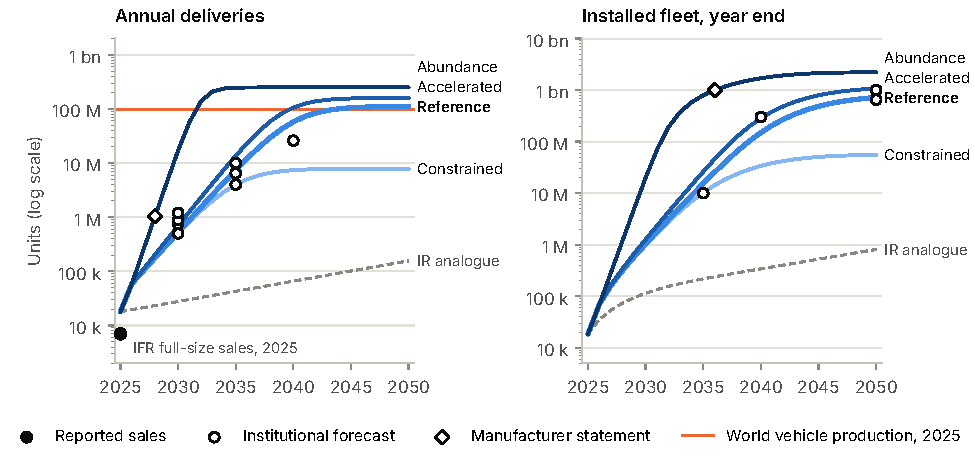
\includegraphics[width=\linewidth]{../figures/out/fig01_trajectories.pdf}
\caption{Annual deliveries and year-end installed fleet by scenario, with published checkpoints. The dashed line is the industrial-robot analogue of \secref{sec:analogue}.}
\label{fig:traj}
\end{figure}

\subsection{Why an industrial-robot analogue is not a scenario}\label{sec:analogue}
A natural way to avoid analyst forecasts is to borrow an observed growth rate from a related market. World industrial-robot installations rose from 254\,000 in 2015 to 603\,000 in 2025 \citep{ifr2026world}, a log-growth rate of 8.65\,\% per year. Applied to the 2025 humanoid anchor, that rate gives \AnaStockFifty\ humanoids in service and \AnaTWhFifty\TWh\ in 2050.

The comparison is shown in Figures~\ref{fig:traj} and~\ref{fig:energy} and is not used as a scenario, for two reasons. The rate is already contradicted by the evidence it would replace: humanoid deliveries grew several-fold between 2024 and 2025 and again into 2026, so an 8.65\,\% path is falsified in its first year. And a mature market's growth rate describes the late, saturating part of a diffusion curve; applied to the first years of a new product it imposes an outcome rather than avoiding one. The analogue is reported because it shows how much of any long-range result is carried by the diffusion phase assumed: the reference case is \AnaRatio\ times larger.

% =====================================================================
\section{Fleet model}\label{sec:fleet}

\subsection{Logistic deliveries}
New technologies that replace or extend an existing activity typically diffuse along an S-shaped curve: slow at first, compounding through a take-off phase, then saturating as the addressable market fills \citep{griliches1957,bass1969,fisherpry1971}. The present model applies that form to annual deliveries rather than to stock:
\begin{equation}\label{eq:logistic}
q_t \;=\; \frac{Q_{\max}}{1+\exp\!\big[-k\,(t-t_m)\big]},\qquad t_m \;=\; 2026 + \frac{1}{k}\ln\!\left(\frac{Q_{\max}}{q_{2026}}-1\right),
\end{equation}
for $t\ge 2026$. Here $Q_{\max}$ is the long-run annual delivery rate, $k$ the ramp rate and $t_m$ the year in which deliveries reach half their ceiling. The midpoint is not a free parameter: it is fixed so that every trajectory passes through the 2026 anchor. Early growth is approximately $e^{k}-1$ per year.

Placing the logistic on deliveries has two advantages over placing it on stock. $Q_{\max}$ is directly comparable with manufacturing quantities, most usefully with world motor-vehicle production of 96.4~million units in 2025 \citep{oica2026}. And the installed stock then follows from deliveries and survival without a separate saturation assumption. A fleet whose deliveries plateau at $Q_{\max}$ approaches a stock of roughly $Q_{\max}$ times the mean service life.

\subsection{Calibration to checkpoints}\label{sec:calib}
Each scenario fits the two free parameters $(Q_{\max},k)$ to a named set of checkpoints $\{y_i\}$ by minimising squared log errors,
\begin{equation}\label{eq:fit}
\min_{Q_{\max},\,k}\; \sum_i \Big[\ln \hat y_i(Q_{\max},k) - \ln y_i\Big]^2,
\end{equation}
where $\hat y_i$ is the model's annual delivery or installed stock in the checkpoint's year, computed with the scenario's other parameters. Log errors treat a factor of two as equally wrong in either direction and keep the large 2050 values from dominating the small 2030 ones. Checkpoints that a scenario is not fitted to are reported afterwards as out-of-fit ratios.

The reference case is fitted to all twelve institutional checkpoints at once. It is a compromise trajectory, and its residuals record how far the published record is from internal consistency. The fitted curve has a ceiling $Q_{\max}$ of \RefQmax\ deliveries per year and $k=\Refk$, equivalent to \Refkpct\,\% early annual growth with a midpoint in \Reftm. Model-to-checkpoint ratios lie between \RefFitMin\ and \RefFitMax, with a geometric mean deviation of a factor of \RefFitGeo. The pattern is systematic. The fitted path sits below three of the four 2030 shipment forecasts, above Wood Mackenzie's 2035 figure (\RefWMSThirtyFive\ for installed stock) and Berg Insight's 2040 shipments (\RefBerg), and below Bank of America's 2040 installed base (\RefBofASForty). It reaches \RefStockFifty\ in 2050, between the Citi (ratio \RefCitiRatio) and Morgan Stanley (\RefMSRatio) views. No smooth trajectory meets all of these together; the reference case is the one that misses them least on a logarithmic scale.

\subsection{Cohorts and exposure}\label{sec:cohorts}
A unit delivered in year $c$ enters service at $\tau_c = c + w$, where $w$ is the mean commissioning point within the year, with a fraction $f$ of deliveries entering the energised fleet. Survival at service age $a$ is Weibull,
\begin{equation}\label{eq:weibull}
W(a) = \exp\!\big[-(a/\lambda)^{\kappa}\big],\qquad \lambda = L/(\ln 2)^{1/\kappa},
\end{equation}
with median life $L$ and shape $\kappa=3$, so the retirement hazard rises with age. The central median life is eight years, with a declared range of five to twelve, bracketing the six-year replacement cycle assumed by Morgan Stanley and the twelve years or more typical of industrial robots. Year-end stock and exposure during year $t$ are
\begin{equation}\label{eq:exposure}
S_t = \sum_{\tau_c<t+1} f\,q_c\,W(t+1-\tau_c),\qquad
RY_{t,c} = f\,q_c\int_{\max(t,\tau_c)}^{t+1} W(u-\tau_c)\,du,
\end{equation}
and the integral has a closed form in the regularised incomplete gamma function. Annual energy is
\begin{equation}\label{eq:energy}
E_t = \sum_{c\le t} RY_{t,c} \sum_{p} \omega_p(c)\, e_p(c,t),
\end{equation}
where $\omega_p(c)$ is the share of cohort $c$ in operating profile $p$ (factory, warehouse, household) and $e_p(c,t)$ the grid-side energy per robot-year of a machine of that vintage and profile in calendar year $t$ (\secref{sec:unit}). Stock never multiplies a full year of energy: a unit commissioned in July contributes half a year before survival adjustment. This is the exposure correction of the 2035 study, now resolved by cohort.

\subsection{Scenarios}\label{sec:scenarios}
The four scenarios are coherent narratives (\tabref{tab:scendef}). Each names the checkpoints its trajectory is fitted to and the machine parameters it changes; every unnamed parameter takes its central value. None is the simultaneous low or high of every input.

\begin{table}[t]
\centering\small
\caption{Scenario definitions: calibration checkpoints and parameters that differ from the central values.}
\label{tab:scendef}
\begin{tabularx}{\linewidth}{@{}l X c c c c c@{}}
\toprule
Scenario & Trajectory fitted to & Household & Hours & SR & Compute & Life \\
 & & 2050 & ratio & ratio & ratio & (yr) \\
\midrule
Constrained & Lowest published path: SAG 2030, Wood Mackenzie 2035 & 0.10 & 1.20 & 0.85 & 1.25 & 8 \\
Reference & All twelve institutional checkpoints, 2030--2050 & 0.40 & 1.50 & 0.75 & 1.50 & 8 \\
Accelerated & Bank of America: 2030 and 2035 shipments, 2040 installed base & 0.55 & 1.75 & 0.70 & 1.75 & 8 \\
Abundance & Tesla 2027 line rate; one billion in service by 2036 & 0.65 & 2.50 & 0.60 & 2.00 & 10 \\
\bottomrule
\end{tabularx}
\end{table}

\emph{Constrained} describes humanoids that remain factory and logistics equipment. The near-term trajectory follows the lowest published forecasts, household adoption stalls at a tenth of deliveries, and utilisation and hardware improve modestly. Fitted exactly to its two checkpoints, it saturates at \ConQmax\ deliveries a year.

\emph{Reference} is the joint fit of \secref{sec:calib}. Household machines rise to two-fifths of 2050 deliveries. Active hours grow by half as autonomy improves and machines move to multi-shift work. Locomotion efficiency improves by a quarter.

\emph{Accelerated} follows the Bank of America trajectory, the most expansive institutional view, in which households become the largest market. Its three checkpoints cannot all be met by one logistic curve. The fitted path is \AccBofAThirty\ of the 2030 figure, \AccBofAThirtyFive\ of the 2035 figure and \AccBofASForty\ of the 2040 installed base.

\emph{Abundance} follows the manufacturer statements: Tesla's line rate as the 2028 delivery level and a billion humanoids in service by 2036. It is fitted exactly and requires $k=\Abuk$, an early growth rate of \Abukpct\,\% per year. That lies outside the declared range of $k$ (0.40--0.80), so Abundance is not part of the sampled uncertainty space of \secref{sec:uncertainty}. It is reported as a stress case: the trajectory that follows if the largest entrant's public targets are met.

% =====================================================================
\section{Unit model to 2050}\label{sec:unit}

\subsection{Inherited structure}
Active power is built from the specific resistance of legged locomotion, $\mathrm{SR}=P/(mgv)$, for which measured values on real platforms range from 0.7 (Cassie) to 2.27 (ASIMO) \citep{kashiri2018}. The active state combines locomotion, manipulation and static posture holding, plus thermal overhead and onboard compute:
\begin{equation}\label{eq:active}
P_a(c) = \big(\phi_L + \phi_M\kappa_M + \phi_S\kappa_S\big)\,\mathrm{SR}(c)\,m\,g\,v\,(1+\tau) + P_c(c),
\end{equation}
where $\phi$ are time shares of an active hour and $\kappa$ the power of manipulation and holding relative to locomotion. With the central parameters of the 2035 study a 2025 factory machine draws \UnitFacPaTwentyFive\,kW when active and consumes \UnitFacTwentyFive\,kWh per robot-year at the grid. The corresponding values for warehouse and household profiles are \UnitWhTwentyFive\ and \UnitHhTwentyFive\,kWh, reproducing Appendix~B of \citet{merilehto2026a} to within 0.3\,\%. The grid-side expression is
\begin{equation}\label{eq:grid}
e = \frac{P_a H + P_r H_r + P_s H_s}{\eta_{\mathrm{ch}}\,\eta_{\mathrm{pk}}}\,(1+d_{\mathrm{dock}})(1+d_{\mathrm{site}}),
\end{equation}
with $H$ active hours, $H_r$ and $H_s$ the hours in connected-ready and deep-sleep states, and the remaining terms the charger and pack efficiencies and the dock and site loss fractions.

\subsection{Time paths to 2050}\label{sec:evolution}
Four declared paths connect the 2025 machine to a 2050 machine. Each moves linearly between 2025 and 2050 with $\pi(x)=\min\{1,\max[0,(x-2025)/25]\}$:
\begin{equation}\label{eq:paths}
\begin{gathered}
\mathrm{SR}(c) = \mathrm{SR}_{0}\big[1+(r_{\mathrm{SR}}-1)\pi(c)\big],\qquad
P_c(c) = P_{c,0}\big[1+(r_{P}-1)\pi(c)\big],\\
H_p(t) = H_{p,0}\big[1+(r_{H}-1)\pi(t)\big],
\end{gathered}
\end{equation}
and the household share of cohort $c$ rises from 5\,\% of 2025 deliveries to $h_{2050}$. Hardware parameters depend on the build year $c$: a robot keeps the efficiency it was built with. Utilisation depends on the calendar year $t$, on the reasoning that autonomy is delivered by software to the whole fleet. The central values are a 25\,\% reduction in specific resistance by 2050 (from 0.80 to 0.60, still three times human walking), a 50\,\% increase in onboard compute, a 50\,\% increase in active hours, and a 40\,\% household share of 2050 deliveries. The household range, 10--65\,\%, spans Morgan Stanley's view of about 8\,\% of the 2050 stock in homes and Bank of America's 62\,\% by 2060. All four are class-A assumptions with declared ranges (Appendix~\ref{app:params}). No efficiency gain is assumed merely because time passes beyond what these paths state.

The 2050 reference factory machine draws \UnitFacPaFifty\,kW when active, works \UnitFacHFifty\ hours a year and consumes \UnitFacFifty\,kWh. The warehouse and household machines consume \UnitWhFifty\ and \UnitHhFifty\,kWh (\figref{fig:unit}, left). Per-robot energy rises despite the efficiency gain because the machine works more hours; \secref{sec:composition} decomposes the net effect.

\begin{figure}[t]
\centering
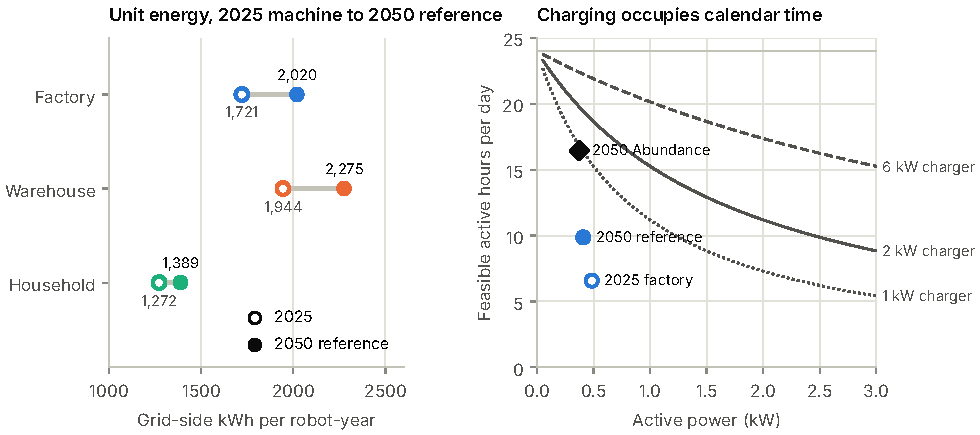
\includegraphics[width=\linewidth]{../figures/out/fig02_unit.pdf}
\caption{Unit energy by operating profile (left) and the charging feasibility frontier of Eq.~(\ref{eq:calendar}) (right).}
\label{fig:unit}
\end{figure}

\subsection{Charging still occupies calendar time}
Higher utilisation brings the charging constraint of the 2035 study into play. Work and the charging needed to replace it must fit within the year,
\begin{equation}\label{eq:calendar}
H + \frac{P_a H}{P_{\mathrm{ch}}\,\eta_{\mathrm{ch}}\eta_{\mathrm{pk}}} \;\le\; 8760,
\end{equation}
which at 2\,kW and the central efficiencies limits a 0.41\,kW machine to about 19 active hours a day (\figref{fig:unit}, right). Sampled worlds that request more hours are capped at the frontier and counted: \MCHCapped\,\% of the hard-bounds experiment and \MCSCapped\,\% of the soft-interval experiment reach it. Round-the-clock operation, a recurring element of manufacturer narratives, requires battery swapping or chargers well above the 2\,kW rating that is the only disclosed humanoid fast-charge figure. The Abundance factory machine, working 6\,000 hours a year (16.4 hours a day), sits just inside the 1\,kW frontier.

% =====================================================================
\section{Results}\label{sec:results}

\subsection{Scenarios}
\tabref{tab:results} and \figref{fig:energy} give the four scenarios. The reference case reaches \RefShipThirtyFive\ deliveries and \RefStockThirtyFive\ installed units in 2035, drawing \RefTWhThirtyFive\TWh\ of grid electricity. By 2050 it reaches \RefShipFifty\ deliveries a year, \RefStockFifty\ in service and \RefTWhFifty\TWh, with a further \RefOffFifty\TWh\ of allocated offboard inference reported separately. Demand grows by a factor of \RatioFiftyThirtyFive\ between 2035 and 2050 because the logistic midpoint, \Reftm, falls between them. Most of the fleet that exists in 2050 is delivered after 2040.

\begin{table}[t]
\centering\footnotesize\setlength{\tabcolsep}{4.2pt}
\begin{threeparttable}
\caption{Scenario results. Peak is the sum of regional unmanaged coincident charging peaks.}
\label{tab:results}
\begin{tabular}{@{}l r r r r r r r r r r@{}}
\toprule
 & \multicolumn{2}{c}{Trajectory} & \multicolumn{3}{c}{2035} & \multicolumn{5}{c}{2050} \\
\cmidrule(lr){2-3}\cmidrule(lr){4-6}\cmidrule(l){7-11}
Scenario & $Q_{\max}$ & $k$ & Deliv. & Stock & TWh & Stock & kWh/ & TWh & Offb. & Peak \\
 & (M/yr) & & (M) & (M) & & (M) & robot-yr & & TWh & (GW) \\
\midrule
\inputtable ../model/outputs/tab_scenarios.tex 
\midrule
\multicolumn{11}{@{}l}{\emph{For comparison}} \\
hre-2.0.0 reference\tnote{a} & -- & -- & 5.0 & 9.9 & \LegacyTWh & -- & -- & -- & -- & -- \\
Industrial-robot analogue & -- & -- & -- & -- & \AnaTWhThirtyFive & 0.8 & -- & \AnaTWhFifty & -- & -- \\
\bottomrule
\end{tabular}
\begin{tablenotes}\footnotesize
\item[a] \citet{merilehto2026a}, reproduced by the present unit model with the inherited fleet inputs.
\end{tablenotes}
\end{threeparttable}
\end{table}

\begin{figure}[t]
\centering
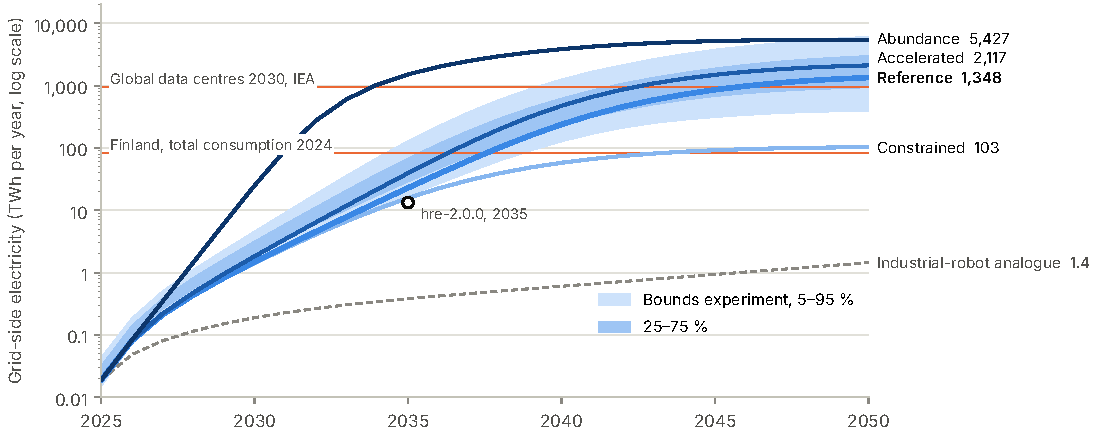
\includegraphics[width=\linewidth]{../figures/out/fig03_energy.pdf}
\caption{Annual grid-side electricity by scenario, 2025--2050. Bands show the 5th--95th and 25th--75th percentiles of the hard-bounds experiment.}
\label{fig:energy}
\end{figure}

The scenarios span a factor of \RatioAbuCon\ in 2050, from \ConTWhFifty\TWh\ in Constrained to \AbuTWhFifty\TWh\ in Abundance. In 2035 they span \ConTWhThirtyFive\ to \AbuTWhThirtyFive\TWh. The Constrained trajectory saturates in the late 2030s at \ConQmax\ deliveries a year and a fleet of \ConStockFifty. Its 2050 demand still exceeds Finland's annual electricity consumption. Accelerated reaches \AccStockFifty\ humanoids and \AccTWhFifty\TWh. Abundance, which passes \AbuStockThirtyFive\ in service by 2035, reaches \AbuStockFifty\ and \AbuTWhFifty\TWh\ by 2050, about \AbuWorldShare\,\% of the world electricity consumption the IEA projects for 2030 (\secref{sec:comparators}).

\subsection{What the machine changes}\label{sec:composition}
Factory and warehouse robots carry most of the reference demand even in 2050, because household machines work fewer hours and arrive later (\figref{fig:composition}, left). Household robots account for \RefHHshare\,\% of 2050 reference energy.

The right panel of \figref{fig:composition} isolates the machine. Holding the reference fleet fixed, a frozen 2025 machine with 2025 duty cycles and a 5\,\% household share would draw \LfA\TWh\ in 2050. Moving to the 40\,\% household share changes this by \LfBd\TWh, since household machines work fewer hours. Locomotion efficiency changes it by \LfCd\TWh, growth in onboard compute by \LfDd\TWh, and the 50\,\% rise in utilisation by \LfEd\TWh, reaching \LfE\TWh. The physical paths largely offset one another: the net change from the frozen machine is less than 8\,\%. The \RatioFiftyThirtyFive-fold growth between 2035 and 2050 is a fleet result.

\begin{figure}[t]
\centering
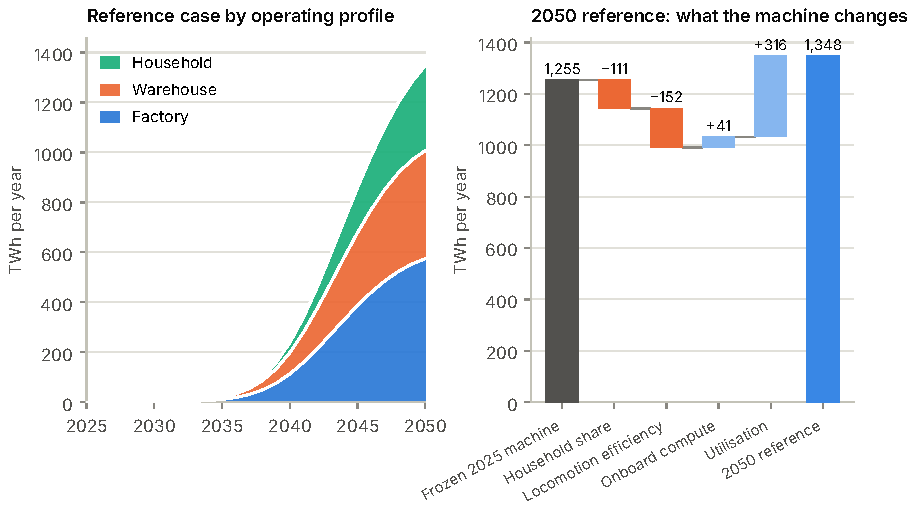
\includegraphics[width=\linewidth]{../figures/out/fig04_composition.pdf}
\caption{Reference-case electricity by operating profile (left) and the effect of each machine path on 2050 demand (right).}
\label{fig:composition}
\end{figure}

\subsection{The 2035 checkpoint}\label{sec:ladder}
The present reference case gives \RefTWhThirtyFive\TWh\ for 2035, \RatioRefLegacy\ times the earlier study's 13.3\TWh. \figref{fig:ladder} walks between the two in single changes. Replacing constant 7\,\% annual attrition with eight-year Weibull cohorts adds \LadBd\TWh, because younger machines survive longer under a rising hazard. Replacing the geometric 30\,000-to-5-million delivery path with the calibrated logistic adds \LadCd\TWh. This is the largest step. It reflects partly evidence published after the earlier study's cutoff (the September 2026 tracker counts and the IDC, SAG and Berg Insight forecasts) and partly forecasts the earlier study did not use (the Bank of America trajectory and the long-range installed-base views that enter the joint fit). Moving the use-case mix from a fixed 25\,\% household share to the rising path adds \LadDd\TWh. Hardware learning to 2035 subtracts \LadEd\TWh. Higher utilisation adds \LadFd\TWh.

The earlier estimate is not contradicted: run on the trajectory its own evidence supported, it reproduces exactly. The difference lies in the deployment record each study is calibrated to, and the size of the step for a record that changed within two months is itself an indication of how firm any single trajectory is.

\begin{figure}[t]
\centering
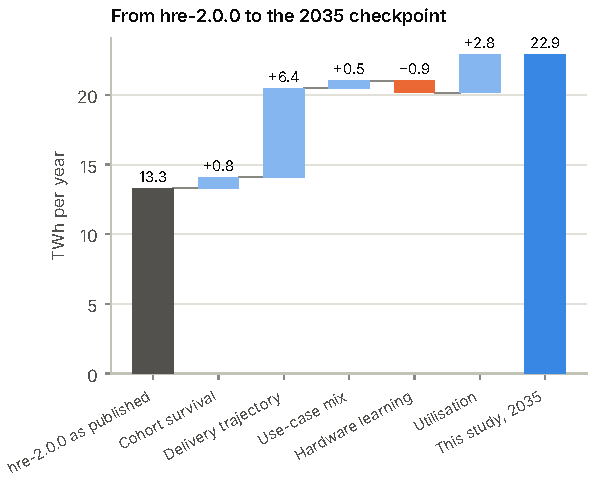
\includegraphics[width=0.66\linewidth]{../figures/out/fig05_ladder2035.pdf}
\caption{From the hre-2.0.0 reference case to the 2035 result of this study.}
\label{fig:ladder}
\end{figure}

\subsection{Charging load and coincident peak}
Annual energy and coincident capacity answer different questions. Charging is resolved in time with the regional local-time shapes of the 2035 study, rotated into UTC (\figref{fig:peaks}). In the 2050 reference case the largest regional coincident peak, China's, is \RefPeakCN\,GW unmanaged. The sum of regional peaks is \RefPeakSum\,GW, falling to \RefPeakSumMan\,GW under the declared managed shape. The simultaneous world load peaks at \RefPeakWorld\,GW. The difference between the sum of regional peaks and the world peak is a time-zone diversity credit that no system operator receives. Under a China-concentrated regional vector, holding 70\,\% of the fleet, China's peak rises to \RefPeakCNconc\,GW. For Accelerated and Abundance the sums of regional peaks are \AccPeakSum\ and \AbuPeakSum\,GW.

The charging energy behind these peaks is the year-end energised stock multiplied by the grid energy per robot-year. The hourly profiles therefore average \PeakStockAvg\,GW, slightly above the \PeakAnnualAvg\,GW implied by annual energy, because year-end stock exceeds mean exposure in a growing fleet. The 2035 study applied a further availability factor of 0.88 at this step. The in-service fraction is already part of the energised stock and standby is already part of the per-robot energy, so that factor is dropped here; on the present basis the hre-2.0.0 reference peak would be \LegacyPeakPresent\,GW rather than 1.09\,GW.

These are fleet-scale descriptors, not network studies. They carry the declared charging shapes of the earlier study, and they show that in every scenario except Constrained humanoid charging would reach tens of gigawatts of coincident load in each accounting region by 2050.

\begin{figure}[t]
\centering
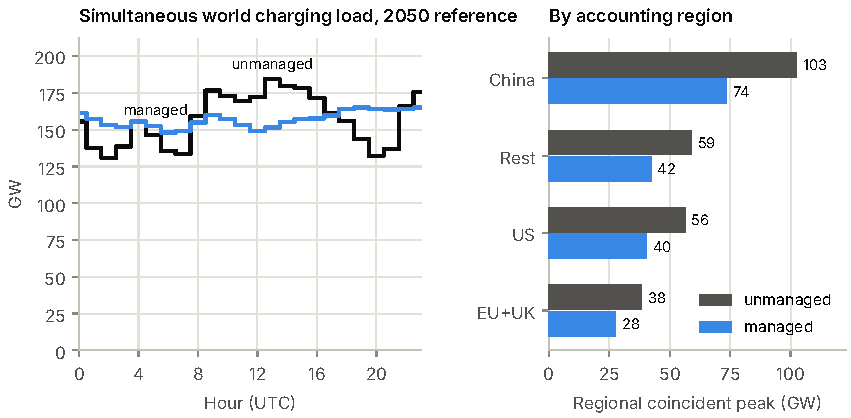
\includegraphics[width=\linewidth]{../figures/out/fig09_peaks.pdf}
\caption{Charging load in the 2050 reference case: world load by hour (left) and regional coincident peaks (right).}
\label{fig:peaks}
\end{figure}

\subsection{Scale against external benchmarks}\label{sec:comparators}
\figref{fig:comparators} places the results among external electricity quantities. These differ in year, geography and boundary, and orient magnitude rather than rank comparable quantities. The IEA puts global electricity consumption at \WorldTwentyFive\TWh\ in 2025 and projects \WorldThirty\TWh\ in 2030 \citep{iea2026elec}. Against the 2030 level, the 2050 reference case is \RefWorldShare\,\%, Accelerated \AccWorldShare\,\% and Abundance \AbuWorldShare\,\%. Global data centres consumed about 485\TWh\ in 2025 and are projected to reach 950\TWh\ in 2030 in the IEA's central projection \citep{iea2026kq} and more than 1\,200\TWh\ in Gartner's \citep{gartner2026}. The 2050 reference case exceeds the IEA's 2030 projection and is comparable in scale to Gartner's, which is stated only as a lower bound; it is more than three times Wood Mackenzie's 2035 estimate for all robotics, industrial arms included \citep{woodmac2026}. At national scale, Fingrid's scenarios put Finnish consumption at 110--162\TWh\ by 2035, from about 85\TWh\ today, with data centres the largest single uncertainty and some 4.5\,GW of data-centre capacity under construction \citep{gasum2026}. Even the Constrained case's 2050 demand would be of the order of a present-day national power system of that size.

\begin{figure}[t]
\centering
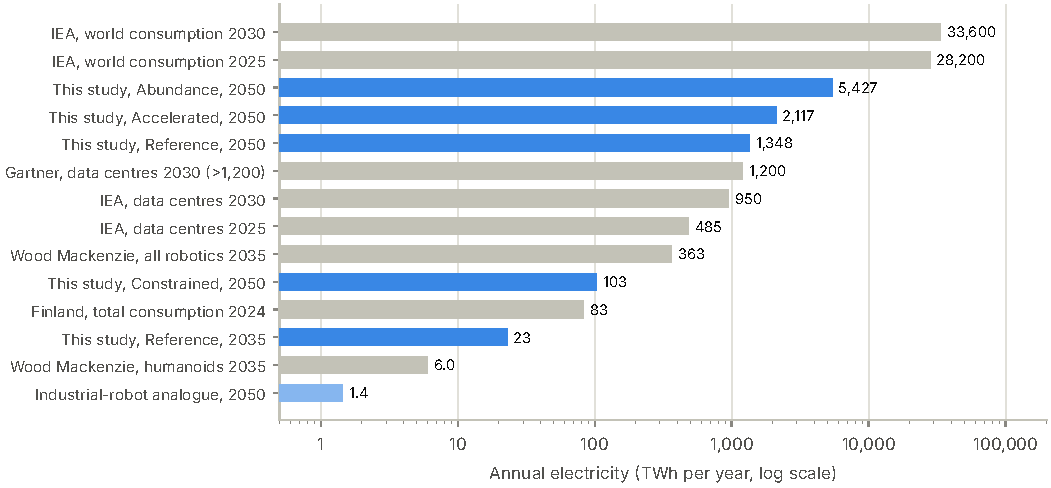
\includegraphics[width=\linewidth]{../figures/out/fig10_comparators.pdf}
\caption{Scenario results against external electricity benchmarks \citep{iea2026elec,iea2026kq,gartner2026,woodmac2026,finnishenergy2025}.}
\label{fig:comparators}
\end{figure}

% =====================================================================
\section{Uncertainty and robustness}\label{sec:uncertainty}

\subsection{The bounds experiment under two readings}
Every input of Appendix~\ref{app:params} is sampled across its declared range, \Draws\ draws per reading, under the two readings used in the 2035 study. Under the \emph{hard-bounds} reading the declared low and high are limits and the sampler is triangular. Under the \emph{soft-interval} reading they are the 10th and 90th percentiles of a two-piece lognormal with its median at the central value. The shipment ceiling is sampled on a logarithmic scale under both readings. Abundance lies outside the declared range of $k$ and is not part of the experiment.

Under hard bounds the 2050 result has a 5th--95th percentile range of \MCHFiftyFive--\MCHFiftyNinetyFive\TWh\ and a median of \MCHFiftyMed\TWh, with an installed base of \MCHStockFive\ to \MCHStockNinetyFive\ (\figref{fig:dist}). Under the soft interval the range widens to \MCSFiftyFive--\MCSFiftyNinetyFive\TWh\ with a median of \MCSFiftyMed\TWh. Including allocated offboard inference, the hard-bounds total range is \MCHTotalFive--\MCHTotalNinetyFive\TWh. For 2035 the hard-bounds range is \MCHThirtyFiveFive--\MCHThirtyFiveNinetyFive\TWh\ with a median of \MCHThirtyFiveMed.

The reference case sits at percentile \MCHPctRef\ of the hard-bounds distribution and \MCSPctRef\ of the soft one. Unlike in the 2035 study, where the reference case fell at percentile 6.5, the central configuration and the distributional summary nearly agree. The main reason is that the dominant input, the shipment ceiling, is sampled on a logarithmic scale with its mode at the value the reference fit produced. Abundance falls at percentile \MCHPctAbu\ of the hard-bounds experiment. A percentile here describes a declared-bounds experiment, not a probability that the world will realise a value \citep{morgan1990}.

\begin{figure}[t]
\centering
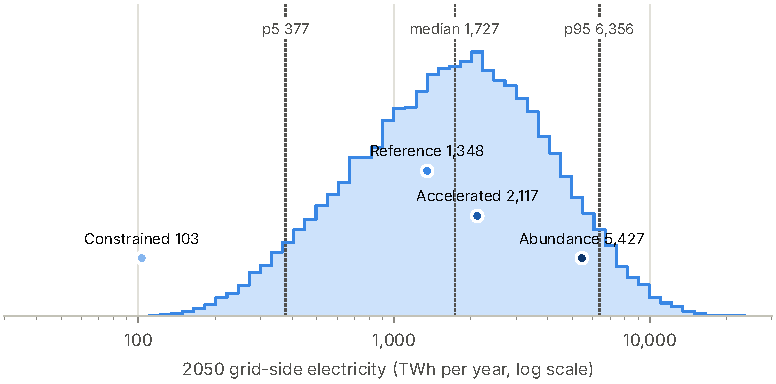
\includegraphics[width=\linewidth]{../figures/out/fig06_distribution.pdf}
\caption{Distribution of 2050 electricity in the hard-bounds experiment.}
\label{fig:dist}
\end{figure}

\subsection{Global variance decomposition}\label{sec:sobol}
First-order and total-effect Sobol indices are estimated by parameter group with Saltelli sampling, the \citet{saltelli2010} first-order estimator and the \citet{jansen1999} total-effect estimator, over \SobolEvals\ model evaluations from a base sample of \SobolBase, with bootstrap confidence intervals. The estimators are validated against the analytically known indices of the Ishigami function in the test suite. Results are given in \figref{fig:sobol} and \tabref{tab:sobol}.

\begin{figure}[t]
\centering
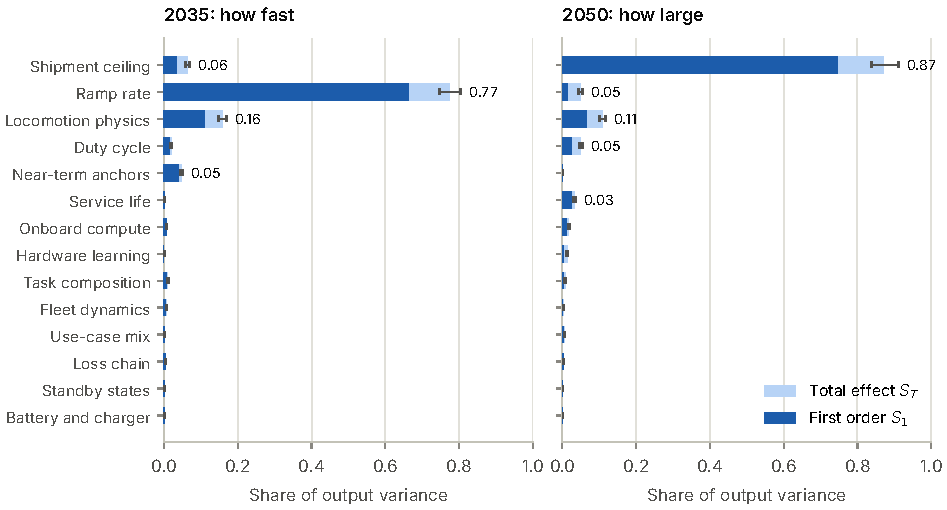
\includegraphics[width=\linewidth]{../figures/out/fig07_sobol.pdf}
\caption{Sobol indices by parameter group, hard-bounds reading. Whiskers show bootstrap 95\,\% intervals on $S_T$.}
\label{fig:sobol}
\end{figure}

The decomposition shows a change of regime. In 2035 the ramp rate $k$ carries most of the variance ($S_T=\SobRampSTThirtyFive$), followed by locomotion physics (\SobLocoSTThirtyFive) and the shipment ceiling (\SobCeilSTThirtyFive). The question in 2035 is how fast the industry grows. In 2050 the shipment ceiling dominates ($S_T=\SobCeilSTFifty$), followed by locomotion physics (\SobLocoSTFifty), duty cycle (\SobDutySTFifty), ramp rate (\SobRampSTFifty) and service life (\SobLifeSTFifty). By 2050 the question is how large the industry becomes. Summed over the nine physical groups, total effects are \SobPhysSTThirtyFive\ in 2035 and \SobPhysSTFifty\ in 2050; total effects overlap, so these sums are upper bounds on the joint contribution. The loss chain, the term energy analysts most often debate, never exceeds $S_T=\SobLossSTThirtyFive$. Interaction effects account for \SobInterThirtyFive\ of the variance in 2035 and \SobInterFifty\ in 2050.

\begin{table}[t]
\centering\small
\caption{Sobol indices by parameter group, hard-bounds reading, ordered by 2050 total effect.}
\label{tab:sobol}
\begin{tabular}{@{}l c c c c@{}}
\toprule
 & \multicolumn{2}{c}{2035} & \multicolumn{2}{c}{2050} \\
\cmidrule(lr){2-3}\cmidrule(l){4-5}
Parameter group & $S_1$ & $S_T$ & $S_1$ & $S_T$ \\
\midrule
\inputtable ../model/outputs/tab_sobol.tex 
\bottomrule
\end{tabular}
\end{table}

The practical reading is that a 2050 humanoid electricity figure is a statement about the eventual size of the humanoid manufacturing industry, converted at roughly 1\,800--2\,500\,kWh per robot-year. Refining the physics narrows the conversion factor, but debate over the long-run figure is mostly debate over the ceiling.

\subsection{Convergence and seed stability}
Across five independent seeds the 2050 hard-bounds median varies by \SeedSpreadMed\,\%, the 5th percentile by \SeedSpreadLo\,\% and the 95th percentile by \SeedSpreadHi\,\%. In both years the bootstrap interval of the leading group's total effect lies well clear of every other group's (\figref{fig:sobol}).

% =====================================================================
\section{Conditions for large-scale adoption}\label{sec:conditions}

\subsection{Industrial scale}
Each trajectory is a statement about manufacturing. \figref{fig:feas} (left) expresses annual deliveries as a multiple of 2025 world motor-vehicle production. The reference case, fitted to the institutional consensus, implies humanoid output overtaking that benchmark in \RefVehYear\ and settling at \RefVehRatio\ times it. Over 2025--2050 it delivers \RefCum\ machines. Accelerated overtakes vehicle production in \AccVehYear; Abundance does so in \AbuVehYear\ and settles at \AbuVehRatio\ times it. Constrained peaks at \ConVehRatio\ of vehicle output.

That the consensus implies a humanoid industry larger than today's automotive industry within two decades is not obvious from any single forecast, and it is the most useful test of the scenarios. Reaching it requires actuator, reducer, sensor and battery supply chains of automotive scale. The reference fleet's 2050 deliveries alone would need about \RefBattery\,GWh of new battery packs a year at the inherited 4\,kWh pack size, and the installed fleet would need about \RefChargerGW\,GW of 2\,kW chargers.

\begin{figure}[t]
\centering
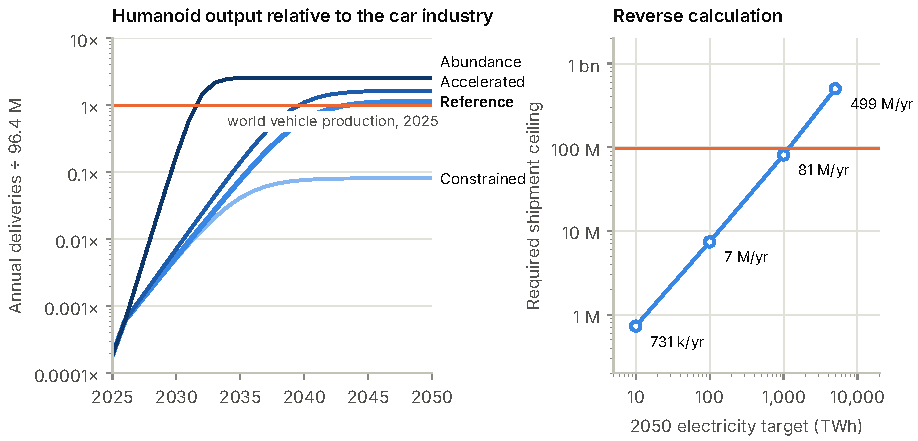
\includegraphics[width=\linewidth]{../figures/out/fig08_feasibility.pdf}
\caption{Humanoid deliveries relative to 2025 world vehicle production \citep{oica2026} (left) and the shipment ceiling required for given 2050 demand (right).}
\label{fig:feas}
\end{figure}

\subsection{Reverse calculation}
A planner may need to know what a given electricity outcome would require rather than what a scenario predicts. Holding every reference parameter fixed except $Q_{\max}$, the ceiling is solved for four 2050 targets (\tabref{tab:reverse}, \figref{fig:feas} right). Ten terawatt-hours requires a ceiling of \RevTenQ\ deliveries a year, about 1\,\% of vehicle production. One thousand requires \RevThousandQ, \RevThousandVeh\ of vehicle production. Five thousand, close to the Abundance outcome, requires \RevFiveThousandQ\ a year, \RevFiveThousandVeh\ times vehicle production, and a fleet of \RevFiveThousandStock. The relationship is close to proportional above about 100\TWh, because by 2050 the fleet is near its saturation level whatever the ramp.

\begin{table}[t]
\centering\small
\caption{Shipment ceiling required for given 2050 electricity demand.}
\label{tab:reverse}
\begin{tabular}{@{}r r r r@{}}
\toprule
2050 target (TWh) & $Q_{\max}$ (M/yr) & Multiple of 2025 vehicle production & 2050 stock (M) \\
\midrule
\inputtable ../model/outputs/tab_reverse.tex 
\bottomrule
\end{tabular}
\end{table}

\subsection{Useful-work economics}
Adoption depends on useful output per unit cost, not on powered-on hours. With installed cost $C$, capital-recovery factor $A(i,L_r)$, annual maintenance $m$ as a fraction of capital, active hours $H$, a human wage $W$, supervision $\alpha$ human hours per robot hour and electricity price $\pi_e$, the break-even condition for $p$ human-equivalent hours of work per robot hour is
\begin{equation}\label{eq:breakeven}
p_{\min} \;=\; \alpha + \frac{C\,[A(i,L_r)+m] + e(H)\,\pi_e}{H\,W}.
\end{equation}
The illustrative inputs are the US May 2025 mean wage for stockers and order fillers, USD~19.01 an hour \citep{bls2026}, an 8\,\% discount rate over eight years ($A=\EcoA$), 10\,\% annual maintenance, 0.1 supervision hours per robot hour and USD~0.15 per kWh. Energy $e(H)$ is recomputed for each duty with the 2050 reference factory machine. Installed costs span USD~15\,000--200\,000. The range covers an average selling price of about USD~29\,600 in 2026, derived from IDC revenue and shipment data as reported by \citet{idc2026}, Bank of America's expectation of a China-built bill of materials below USD~17\,000 by 2030 \citep{bofa2026}, and Morgan Stanley's mid-century price of USD~50\,000 in high-income markets \citep{ms2025}.

\begin{table}[t]
\centering\small
\caption{Break-even productivity $p_{\min}$ (human-equivalent hours per robot hour) and electricity share of annual ownership cost.}
\label{tab:econ}
\begin{tabular}{@{}r c c c c@{}}
\toprule
Installed cost (USD) & 2\,400 h/yr & 3\,600 h/yr & 6\,000 h/yr & Electricity share at 3\,600 h (\%) \\
\midrule
\inputtable ../model/outputs/tab_econ.tex 
\bottomrule
\end{tabular}
\end{table}

At USD~30\,000 and 3\,600 hours a year a robot breaks even at \EcoPminThirtyKThreeSix\ human-equivalent hours per robot hour (\tabref{tab:econ}, \figref{fig:econ}). Only the most expensive and least utilised case, USD~200\,000 at 2\,400 hours, requires more than one (\EcoPminTwoHundredKTwoFour). Across all cases electricity is \EcoElecShareMin--\EcoElecShareMax\,\% of annual ownership cost; at USD~30\,000 and 3\,600 hours it is about USD~\EcoElecCostThreeSix\ a year. Under the stated cost and tariff assumptions, electricity is therefore a small component of annual ownership cost, and capital cost, achievable productivity and supervision weigh far more on the break-even condition. This does not establish that adoption is insensitive to electricity prices: marginal deployments may remain price-sensitive, and the incentive to shift charging in time is a separate question. Price responsiveness and charging flexibility are not estimated here. A related argument has been made for data centres, whose high margins limit their incentive to offer demand flexibility and shift the need for flexibility to other market participants \citep{gasum2026}; whether humanoid fleets behave similarly is an open question.

\begin{figure}[t]
\centering
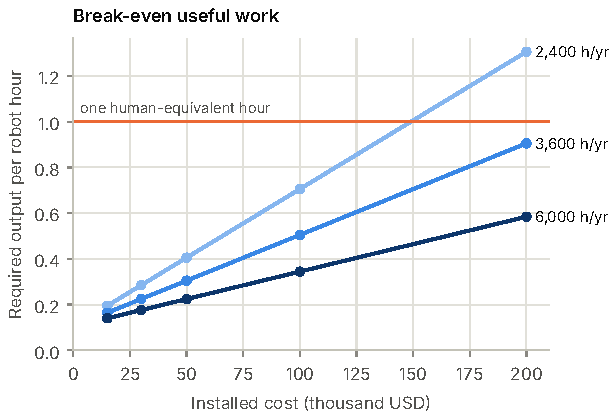
\includegraphics[width=0.64\linewidth]{../figures/out/fig11_economics.pdf}
\caption{Break-even useful work per robot hour against installed cost.}
\label{fig:econ}
\end{figure}

\subsection{Reading the Abundance case}
Abundance is the outcome of taking the stated targets of the largest entrant at face value. It requires early growth of about \Abukpct\,\% a year, humanoid output above world vehicle production by \AbuVehYear, \AbuCum\ deliveries by 2050, and machines working 6\,000 hours a year. Each of these is a measurable condition. Deliveries of 1~million in 2028, 17~million in 2030 and an industry of automotive scale by the early 2030s would be visible years ahead in supplier capacity, battery orders and grid-connection requests. The case is reported so that planners can identify those signals early, not because the evidence favours it: it lies outside the declared range of every institutional forecast.

% =====================================================================
\section{What this model does not improve}\label{sec:notimproved}
The unit model is no better constrained than it was in the 2035 study. Task composition, the manipulation and holding ratios and the standby powers rest on declared values and a single vendor claim. The time paths of \secref{sec:evolution} add four further declared assumptions. Their small variance shares mean that they matter less than the fleet under the declared ranges. They do not mean that the values are well known.

The fleet model makes the deployment record explicit; it does not make it more reliable. The logistic form is a convention with a long empirical history in technology diffusion, but it imposes symmetric take-off and saturation. A market that saturates slowly in households after fast industrial adoption would follow a different shape. Two-wave or Bass-type forms with separate industrial and household potentials are a natural extension once household deliveries are observed. The checkpoints themselves are analyst products drawing on an overlapping public record. Their mutual inconsistency is informative, but their agreement would not be independent corroboration.

\section{Limitations}\label{sec:limits}
\textbf{The near-term anchor is short.} The model is pinned to a 2026 delivery total that is only half observed. If 2026 shipments turn out well below 45\,000 or above 90\,000, every trajectory shifts.

\textbf{The ceiling is an assumption with an industrial meaning.} $Q_{\max}$ is fitted or sampled, never observed. Its comparison with vehicle production is the main check on its plausibility, and the reverse calculation exists to make that check easy to apply.

\textbf{The long-range reference result rests on two installed-base views.} Morgan Stanley's and Citi's 2050 figures are the only checkpoints beyond 2040. Removing both from the reference fit lowers the fitted ceiling to \NoSecQmax\ a year, the 2050 installed base to \NoSecStock\ and 2050 demand to \NoSecTWh\TWh, while 2035 demand moves only to \NoSecTWhThirtyFive\TWh. The near-term result is robust to their exclusion. The long-range reference result is not, and it should be read together with this sensitivity.

\textbf{No household duty-cycle data exist.} The household profile inherits the 2035 study's 1\,095 active hours and its connected-ready share. Household machines that stay connected and ready for most of the day would draw more standby energy than assumed.

\textbf{Peak results are fleet descriptors.} No feeder topology, state-of-charge distribution or charger queueing is represented. The managed shape is a declared profile, not an optimised dispatch.

\textbf{Electricity only.} No emissions, cost-of-supply, capacity-adequacy or life-cycle result follows from this work.

% =====================================================================
\section{Conclusion}\label{sec:conclusion}
Calibrated to the published record of October 2026, a global humanoid fleet of \RefStockFifty\ machines draws \RefTWhFifty\TWh\ of grid-side electricity in 2050 in this study's reference case. Across the declared bounds the range is \MCHFiftyFive--\MCHFiftyNinetyFive\TWh. The 2035 checkpoint is \RefTWhThirtyFive\TWh, higher than the earlier estimate because the deployment record it is calibrated to is broader and more recent. At the scale of the reference case, humanoid robots would draw electricity comparable in scale to published projections for all global data centres in 2030, with a regional coincident charging peak of the order of \RefPeakCN\,GW in the largest market.

Three observations may carry beyond the subject. The first is that the uncertainty changes character over the horizon: the near term is governed by how fast an industry ramps and the long term by how large it becomes, and the physics of the machine, carefully constrained, contributes about a fifth of the variance in either. The second is that published forecasts can be tested against one another by asking what single trajectory would satisfy them. Here no trajectory does, and the best compromise implies a humanoid industry larger than today's car industry by the mid-2040s. That implication is a more useful planning signal than any individual number. The third is that the choice of diffusion phase is the largest assumption in the analysis. A mature-market growth rate applied to a new technology yields \AnaTWhFifty\TWh; the evidence-calibrated take-off yields roughly a thousand times more. A study that does not state which phase it assumes has not stated its main assumption.

The binding constraint on this estimate is no longer the absence of a humanoid power trace, though that absence remains. It is that the size of the humanoid industry in 2040 is not yet observable. The relevant evidence will appear well before 2050: delivery counts, supplier capacity, battery contracts and connection requests. The framework released with this paper can be updated as each arrives.

% =====================================================================
\section*{Data and code availability}
The model source, executable parameter set, generated outputs, figure code and test suite are archived at release v3.0.0 of \url{https://github.com/juhanimerilehto/future2050/tree/v3.0.0}, the exact source that produced this manuscript. The 2035 study and its reproducibility packet are archived at \url{https://doi.org/10.5281/zenodo.22538130} and \url{https://doi.org/10.5281/zenodo.22729903}. Every model-derived number in the text, tables and figures is generated by the model run, so the text cannot drift from the outputs \citep{pfenninger2017}. A full rerun from a clean checkout is:
\begin{verbatim}
python model/run_all.py --draws 50000 --sobol-n 8192
python model/make_numbers.py
python -m unittest discover -s model/tests
python figures/make_figures.py
latexmk -cd -pdf paper/humanoid_electricity_2050.tex
\end{verbatim}
Only Python with NumPy, SciPy and Matplotlib is required. The run is deterministic given the recorded seeds. The parameter file has SHA-256 prefix \texttt{\ParamsSha} and the core model \texttt{\CoreSha}. The test suite checks reproduction of the hre-2.0.0 unit table and reference case, stock--exposure consistency, the 2026 anchor, monotonicity in the shipment ceiling, exact fits of the two exactly identified scenarios and the Ishigami validation of the Sobol estimators.

\bibliographystyle{plainnat}
\bibliography{references}

% =====================================================================
\appendix
\section{Parameter set}\label{app:params}
\tabref{tab:params} lists every parameter with its declared low, central and high values, evidence class, variance group and anchor. Parameters for the 2025 machine are those of \citet{merilehto2026a}; time paths and fleet parameters are new.

{\small
\setlength{\tabcolsep}{4pt}
\begin{longtable}{@{}>{\raggedright\arraybackslash}p{3.9cm} r r r l >{\raggedright\arraybackslash}p{2.6cm} >{\raggedright\arraybackslash}p{3.7cm}@{}}
\caption{Parameter set. Classes: M measured, V vendor claim, S official statistic, F forecast, B benchmark, A assumption.}\label{tab:params}\\
\toprule
Parameter & Low & Central & High & Class & Group & Anchor \\
\midrule
\endfirsthead
\toprule
Parameter & Low & Central & High & Class & Group & Anchor \\
\midrule
\endhead
\inputtable ../model/outputs/tab_params.tex 
\bottomrule
\end{longtable}}

\section{Published checkpoints}\label{app:checkpoints}
\begin{table}[H]
\centering\footnotesize
\setlength{\tabcolsep}{4pt}
\caption{Published checkpoints. Access: P verified in the publisher's document, S secondary reporting only.}
\label{tab:checkpoints}
\begin{tabular}{@{}l c l r c c l r@{}}
\toprule
Source & Year & Quantity & Value & Class & Access & Fitted by & Ref.\ ratio \\
\midrule
\inputtable ../model/outputs/tab_checkpoints.tex 
\bottomrule
\end{tabular}
\end{table}

\end{document}
